\section{Grundlagen}
\label{sec:grundlagen}

\subsection{Threads}
\label{subsec:threads}
Ein Thread ist ein Ausführungsstrang innerhalb eines Prozesses zur Abarbeitung eines Programms.
Jegliche Threads die durch Java-Code erzeugt werden oder von der JVM intern genutzt werden,
sind in der HotSpot-JVM als \verb|Kernel-Threads| implementiert
und bieten Entwicklern verhältnismäßig leichten Zugriff auf parallele Programmierung und Synchronisation von Threads.
\parencite[Absatz Thread Management]{OpenJDKHotspotOverview}

\subsubsection{Kernel-Threads}
\label{subsubsec:kernel-threads}
Als \verb|Kernel-Threads|\footnote{Auch als nativer Thread bezeichnet} werden Threads bezeichnet, deren Ablaufplanung vom Betriebssystem übernommen wird.
Konkret bedeutet das, dass die Zuweisung der Rechenzeit für einen Thread sowie die Threadwechsel (siehe \ref{subsubsec:threadwechsel})
vom Scheduler \& Dispatcher des Kernels geplant und durchgeführt werden.

Mindestens ein \verb|Kernel-Thread|, der \verb|Main-Thread|, existiert innerhalb eines Prozesses. Kernel-Threads innerhalb eines Prozesses
teilen sich Speicheradressräume, Datei-Handles und Netzwerkverbindungen.
Aus diesem Grund ist die Kommunikation zwischen \verb|Kernel-Threads| eines Prozesses deutlich einfacher und performanter
als Interprozesskommunikation.

Allerdings muss eine eventuelle Synchronisation der Threads erfolgen, um gleichzeitige Zugriffe auf dieselbe Ressource zu verhindern
(Deadlock).
Da Kernel-Threads zudem nur über wenige Ressourcen verfügen (Stack, Registerinhalte, Befehlszähler) sind sie, im Vergleich zu Prozessen,
verhältnismäßig günstig zu erstellen und zu zerstören.\parencite[Kapitel 2.2.5]{Tanenbaum2016}

\subsubsection{User-Threads}
\label{subsubsec:user-threads}
Die Funktionalität von \verb|User-Threads| \footnote{Auch als Fiber oder virtueller Thread bezeichnet} ist,
im Gegensatz zu \verb|Kernel-Threads|,
nicht im Kernel implementiert sondern in einer Programmbibliothek im Benutzeradressraum des Betriebssystems.
Da sich das Scheduling-System des Kernels nicht um die Verwaltung solcher Threads kümmern kann, muss dies durch einen eigenen Scheduling-Algorithmus
der jeweiligen Laufzeitumgebung des Programms übernommen werden.
Ein Vorteil dieser Vorgehensweise ist die Möglichkeit, die Schedulingstrategie individuell an die Arbeitslast des Programms anzupassen.

Im Gegensatz zu \verb|Kernel-Threads| kann einem \verb|User-Thread|, der einen blockierenden Systemaufruf macht,
aber vom Scheduler des \verb|Betriebssystems| nicht die Kontrolle über die CPU entzogen werden, da der gesamte Prozess blockiert wäre.
Aus Sicht des Kernels existiert nämlich lediglich der Main-Thread des Prozesses und dieser
führt einen blockierenden Aufruf aus. \footnote{Hier könnte lediglich, abhängig von der Schedulingstrategie des Kernels, ein Prozesswechsel stattfinden}

In Folge der Blockade des Main-Threads kann dieser auch das Scheduling der Laufzeitumgebung nicht ausführen, weswegen während dieser
Zeit auch kein anderer \verb|User-Thread| ausgeführt wird.

Eine Lösung für dieses Problem ist die Nutzung einer asynchronen, nicht-blockierenden API für \gls{io}-Operationen(*)
seitens der Anwendung.
Dadurch wird statt des Main-Threads lediglich der auszuführende \verb|User-Thread| blockiert und dem aufrufenden Main-Thread
sofort die Kontrolle zurückgegeben. Mit der richtigen Schedulingstrategie kann in der Zwischenzeit direkt ein
weiterer \verb|User-Thread| ausgeführt werden. \parencite[Kapitel 2.2.4]{Tanenbaum2016}
Das Prinzip von nicht-blockierenden I/O-Operationen ist im Rahmen dieser Arbeit von hoher Relevanz und wird in Kapitel \ref{subsec:nonblocking-i/o}
genauer erläutert.

\subsubsection{Threadwechsel}
\label{subsubsec:threadwechsel}
Sobald die Schedulingstrategie eines Schedulers erfordert das ein Thread die Kontrolle einer \glsuseri{logische CPU}(*) an
einen anderen Thread abgeben muss, wird von einem \verb|Kontextwechsel| in Form eines \verb|Threadwechsels| gesprochen.
Ein Threadwechsel kann durch eine Reihe von Ereignissen ausgelöst werden:
\begin{enumerate}
  \item Terminierung eines Threads
  \item Warten auf das Ergebnis einer synchronen I/O-Operation
  \item Verbrauch der zugewiesenen Rechenzeit (Zeitscheibe)
  \item Geringere Priorisierung
  \item Freiwillige Abgabe der CPU-Kontrolle (kooperativ)
\end{enumerate}

Insbesondere das 2. Ereignis ist im Rahmen dieser Arbeit von besonderem Interesse und wird in Kapitel \ref{subsec:blocking-i/o} thematisiert.

Während bei einem Kontextwechsel von Prozessen (Prozesswechsel) der gesamte Programmkontext (Adressräume, Inhalt der CPU-Register,
Seitentabelle, geöffnete Dateien und Metainformationen)
gewechselt werden muss, wird bei einem Threadwechsel lediglich der Inhalt der CPU-Register (inklusive Programmzähler und Stack-Pointer)
ersetzt.\parencite{Mosberger2002}

Da der Threadwechsel im Fall von \verb|Kernel-Threads| durch Systemaufrufe, also vom Kernel des Betriebssystems, ausgeführt werden muss, entsteht
bei einem Threadwechsel dennoch ein messbarer Zeitverlust.
Dies ist durch die geringe Geschwindigkeit und den Overhead des notwendigen, vom Dispatcher ausgelösten, Softwareinterrupts bedingt.
Der Softwareinterrupt erfolgt um die Programmausführung im Benutzer-Modus zu unterbrechen.
Dadurch wird die Ausführung der jeweiligen Interrupt Service Routine (ISR) im
Kernel-Modus (Kontextwechsel auf privilegierten Ring 0) erzwungen sowie auf dessen Beendigung gewartet.

Da sich \verb|User-Threads| komplett im Benutzeradressraum befinden, sind Threadwechsel
bei ihnen extrem effizient und deutlich schneller als bei \verb|Kernel-Threads|, da keinerlei Interaktion mit dem Kernel erfolgt.

Solche Threadwechsel werden als virtuelle Threadwechsel bezeichnet.
Der Prozess führt eine Thread-Tabelle mit, in welcher der gesamte Thread-Kontext gespeichert ist.
Bei einem virtuellen Threadwechsel wird der Thread-Kontext des aktiven \verb|User-Threads| in dieser Tabelle gespeichert, und anschließend der Kontext
des nächsten Threads daraus in die Maschinen-Register geladen.
\parencite[Kapitel 2.4.6 und 2.2.4]{Tanenbaum2016}
\newpage
\subsection{Blocking I/O}
\label{subsec:blocking-i/o}
Bei der herkömmlichen synchronen Ausführung von I/O-Operationen blockiert der entsprechende Funktionsaufruf die Ausführung des
Threads bis die Operation abgeschlossen ist. Das Abschließen der Operation kann zwischen wenigen Millisekunden (Zugriff auf die Festplatte),
einigen Sekunden (Abrufen eines Service oder komplexen Queries) oder länger (bei Benutzer-Interaktion) dauern.
Sobald ein Thread blockiert wird, wird er vom Kernel des Betriebssystems in den Sleep- bzw. Waiting-Zustand versetzt.
Wie bereits in Kapitel \ref{subsubsec:threadwechsel} erwähnt, erfolgt ein Threadwechsel sobald der momentane Thread in einen solchen Zustand
versetzt wird.
Diese Art des Aufrufes einer I/O-Operation wird daher als \verb|Blocking I/O| bezeichnet.
Aus diesem Umstand wird schnell ersichtlich, dass ein auf \verb|Blocking I/O| basierender Webserver nicht in der Lage ist
performant mehrere Anfragen in einem Thread zu bearbeiten, denn sobald der Thread blockiert, werden alle weiteren zu bearbeitenden Anfragen
auch blockiert.
\subsubsection{Thread per Request}
\label{subsubsec:thread per request}
Daher binden \Gls{servlet-container}(*) üblicherweise jede vom Webserver weitergeleitete HTTP-Anfrage an jeweils einen
Thread im Servlet-API, welcher die jeweilige Anfrage imperativ abarbeitet, daher auch als \verb|Worker thread| bezeichnet.
Sie nutzen das \verb|Thread per request|-Modell.
Der auszuführende Code ist in diesem Ansatz, wie in Abbildung \ref{fig:blocking_thread_per_request} dargestellt,
an den jeweiligen Thread gekoppelt und falls ein Thread durch eine I/O-Operation blockiert wird, werden
die anderen Threads bzw. die zu bearbeitenden Anfragen davon nicht direkt beeinflusst.
\begin{figure}[ht!]
  \centering
  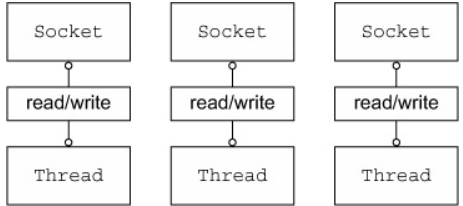
\includegraphics[width=0.6\textwidth]{Blocking-IO-Thread-Per-Request-MultiThread}
  \caption{Thread per Request mit Blocking I/O}
  \label{fig:blocking_thread_per_request}
\end{figure}

Das Erstellen eines neuen Threads für jede Anfrage erzeugt besonders bei vielen kurzlebigen Anfragen einen hohen Overhead und
verwendet unvorhergesehen viele Ressourcen des Betriebssystems. Dies kann gerade bei potentiell hohen Lasten zu erheblichen Problemen
führen.
Aus diesem Grund wird das \verb|Thread per request|-Modell in der Regel um einen \verb|Threadpool| erweitert.
Dabei wird eine begrenzte Anzahl an Threads bereits im Vorfeld erstellt und wiederverwendet.
Dadurch amortisieren sich die Kosten der Erstellung der Threads während der Laufzeit und die benötigten Ressourcen werden begrenzt.
Anfragen können solange parallel ausgeführt werden bis die Anzahl der gleichzeitigen Anfragen die Anzahl der Threads im \verb|Threadpool|
übersteigt.
Ab diesem Punkt müssen eingehende Anfragen solange warten bis ein Thread wieder verfügbar ist.
Der erreichbare Grad der Parallelität ist bei diesem Ansatz in jedem Fall durch die Größe des Threadpools begrenzt.
\newpage
\subsection{Non-blocking I/O}
\label{subsec:nonblocking-i/o}
APIs die auf \verb|Blocking I/O| basieren , blockieren den Thread bis die Operation abgeschlossen ist und verursachen somit
immer einen Threadwechsel.
Funktionsaufrufe mit nicht-blockierenden, asynchronen Ressourcenzugriffen kommen hingegen sofort zurück und blockieren den Thread nicht.
Dieser kann dadurch den weiteren Code des Programms ausführen bzw. die nächste Anfrage bearbeiten.
Sobald das Ergebnis des Zugriffs bereit ist, wird der aufrufende Thread darüber informiert.
Diese Art der Ressourcenzugriffe wird als \verb|Non-blocking I/O| bezeichnet.

Die Grundlage für diese Funktionsweise wird durch einen Mechanismus namens \verb|Synchronous Event Demultiplexing|
bzw. \verb|Event notification API| von jedem modernen Betriebssystem bereitgestellt.

\subsubsection{Synchronous Event Demultiplexing}
\label{subsubsec:event demultiplexing}
Der Begriff Demultiplexing beschreibt das Aufteilen eines, aus mehreren Signalen bestehenden, Signals
in seine ursprünglichen Komponenten.

Mit diesem Mechanismus lässt sich eine endliche Menge aus Ressourcen, wie Sockets oder Dateihandles, beobachten.
Sobald eine I/O-Operation, die auf einer der Ressourcen ausgeführt wurde, abgeschlossen ist, gibt der Demultiplexer eine Menge aus Events
zurück. Deren Inhalte geben Auskunft über den Zustand der Ressource.\newline
\verb|Synchronous Event Demultiplexing|, auch als \verb|Event notification API| bezeichnet, wird unter Linux durch \verb|epoll|, unter BSD durch
\verb|kqueue| und unter
Windows durch \verb|IOCP| bereitgestellt.\footnote{Auf alten Systemen wird als Fallback die POSIX-Funktion \textit{select()} genutzt.}

2002 wurde Unterstützung für nicht-blockierende I/O-Operationen in Java mit dem \verb|java.nio|-Paket eingeführt.
Dieses Paket basiert auf den genannten Betriebssystem-Schnittstellen und abstrahiert diese.\parencite{OpenJDKNIO}
Dabei ist \verb|java.nio.channels.selector| der Dreh- und Angelpunkt und gibt Auskunft darüber, welche
beobachteten Ressourcen bereit für I/O-Operationen sind.

Abbildung \ref{fig:nonblocking_single_thread} stellt dar, wie mehrere Ressourcen über die
\verb|java.nio|-APIs überwacht werden können.

Im Gegensatz zum beschriebenen \verb|Thread per request|-Modell, können durch \newline\verb|Non-blocking I/O|
mehrere Anfragen parallel von einem Thread verarbeitet werden, daher die Bezeichnung \verb|Single Threaded|-Modell.
Dies resultiert in einer geringeren Anzahl an benötigten Threads und demnach auch in weniger Threadwechseln.
Darüber hinaus wird die Möglichkeit eines gleichzeitigen Ressourcenzugriffs von mehreren Threads eines Prozesses
durch die Nutzung eines einzigen Threads unterbunden, weswegen eine Thread-Synchronisation nicht erforderlich ist.

Der Aufruf des \verb|Synchronous Event Demultiplexers| ist blockierend (daher auch der Zusatz \verb|Synchronous|)
und zwar solange bis mindestens eine Ressource bereit für eine I/O-Operation ist
\footnote{Ein typischer Polling-Algorithmus würde aufgrund der geringen Verfügbarkeit der Ressourcen
  viel CPU-Rechenzeit verschwenden}.
Sobald dies passiert wird der Aufruf beendet und eine Menge aus Events wird an den Aufrufer zurückgegeben.
\begin{figure}[ht!]
  \centering
  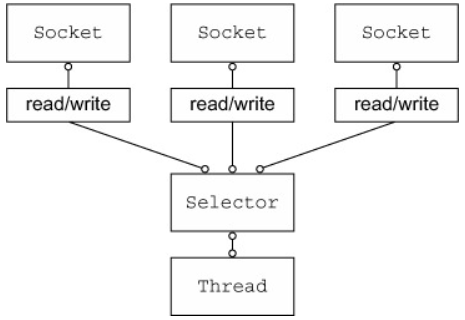
\includegraphics[width=0.6\textwidth]{Nonblocking-IO-EventNotificationAPI-SingleThread}
  \caption{Non-blocking I/O durch java.nio.channels.selector \parencite{NettyInAction}}
  \label{fig:nonblocking_single_thread}
\end{figure}

\subsubsection{Event Loops}
\label{subsubsec:event loops}
Ein beliebtes Modell für die Verarbeitung von asynchronen Events ist die \textit{Event Loop}, die in Abbildung \ref{fig:eventloop} dargestellt wird.
\begin{figure}[ht!]
  \centering
  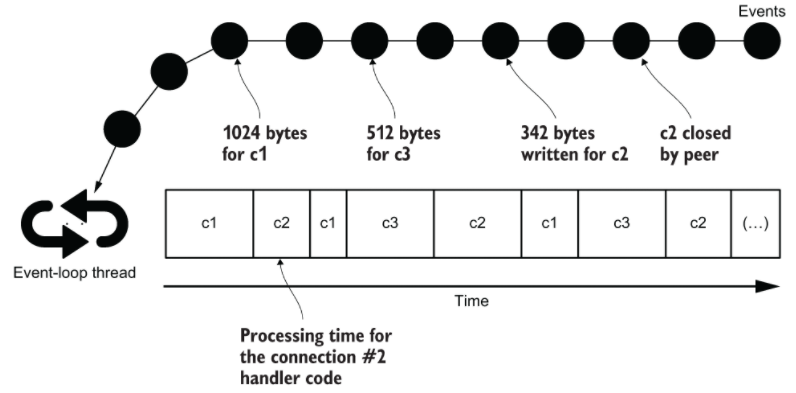
\includegraphics[width=1.0\textwidth]{EventLoop}
  \caption{Exemplarische Abbildung einer Event Loop. \parencite[Kapitel 1.7]{Ponge2020}}
  \label{fig:eventloop}
\end{figure}

Sobald ein Event entsteht, wird es einer Warteschlange (Queue) in der Event Loop hinzugefügt.
Solange der ausführende Thread aktiv ist und die Queue Events enthält, wird in einer Schleife das nächste Event
abgerufen und vollständig verarbeitet bevor die nächste Iteration beginnt.

Dies können beispielsweise I/O-Events sein, die signalisieren das Daten bereit zur Weiterverarbeitung sind,
aber auch jegliches andere Event.
Eine Event Loop wird in der Regel auf einem einzigen Kernel-Thread, dem \verb|IO thread| oder \verb|Event loop thread|,
ausgeführt. Daher darf das Verarbeiten von Events keine blockierenden oder zeitintensiven Operationen beinhalten.
Event Loops wurden zuerst vorrangig in den JavaScript-Engines von Webbrowsern,
und später auch in der Node.js-Laufzeitumgebung, als Basis ihres Nebenläufigkeitsmodells genutzt.
Da JavaScript kein Multithreading unterstützt \parencite{MozillaEventLoop} ist es erforderlich jegliche I/O-Operationen und
Event Handler auf nicht-blockierende Art in einem einzigen Thread auszuführen.\parencite{NodeJSEventLoop}
Für ein laufendes Programm muss der, in Kapitel \ref{subsubsec:event demultiplexing} beschriebene
\newline
\verb|Synchronous Event Demultiplexing|-Mechanismus natürlich kontinuierlich aufgerufen werden.
Wie ein Synchronous Event Demultiplexer während der
gesamten Programmlaufzeit aktiv ist und dessen zurückgegebene Events in einer \verb|Event Loop| verarbeitet werden,
wird in Listing \ref{lst:EventLoop_Pseudocode} als Pseudocode dargestellt.
\newline

\begin{lstlisting}[caption=Einfaches Pseudocode-Beispiel für Synchronous Event Demultiplexing mit Event Loop,
captionpos=b, label=lst:EventLoop_Pseudocode]
//add resources to a data structure and associate them with a specific operation
watchedList.add(socketA, FOR_READ)
watchedList.add(fileB, FOR_READ)
//Note: this call is synchronous and blocks until
//a resource is ready for an i/o-operation
while (events = demultiplexer.watch(watchedList)) {
	// event loop -  process the returned events from the demultiplexer
	for (event of events) {
		// This read will never block and will always return data
		// The resource is guaranteed to be ready for read
		data = event.resource.read()
		if (data == RESOURCE_CLOSED) {
			// the resource was closed, remove it from the watched list
			demultiplexer.unwatch(event.resource)
		} else {
			// some actual data was received - process it 
			// don't block here with a long running operation
			consumeData(data)
		}
 }
}
\end{lstlisting}
Zu Beginn werden die Ressourcen und die darauf auszuführenden Operationen der \verb|watchedList| hinzugefügt.
Diese Liste an Ressourcen wird vom Demultiplexer überwacht. Sobald eine der Ressourcen bereit
für die jeweilige Operation ist, gibt der Demultiplexer eine Menge aus Events zurück die anschließend in einer
Event Loop iteriert wird. Dabei wird der Inhalt der Events gelesen und, falls die Ressource
geschlossen wurde, die Ressource von der \verb|watchedList| entfernt oder der Inhalt in \verb|consumeData| weiterverarbeitet.
\parencite[Event Demultiplexing]{NodeJSDesignPatterns}

\newpage
\subsubsection{Reactor-Pattern}
\label{subsubsec:reactor_pattern}
Das \verb|Reactor-Pattern| ist eine spezielle Form der beschriebenen Algorithmen und kombiniert diese.
Das Modell wurde bereits 1995 beschrieben.\parencite{SchmidtReactorPattern}
Die Hauptidee besteht darin, jedem Event einer Ressource einen Event-Handler zuzuordnen.
Dieser wird aufgerufen sobald das Event entsteht und von der \verb|Event Loop| abgearbeitet wird.
Der grundlegende Aufbau und die Funktionsweise wird in Abbildung \ref{fig:reactor_pattern} dargestellt.
\begin{figure}[H]
  \centering
  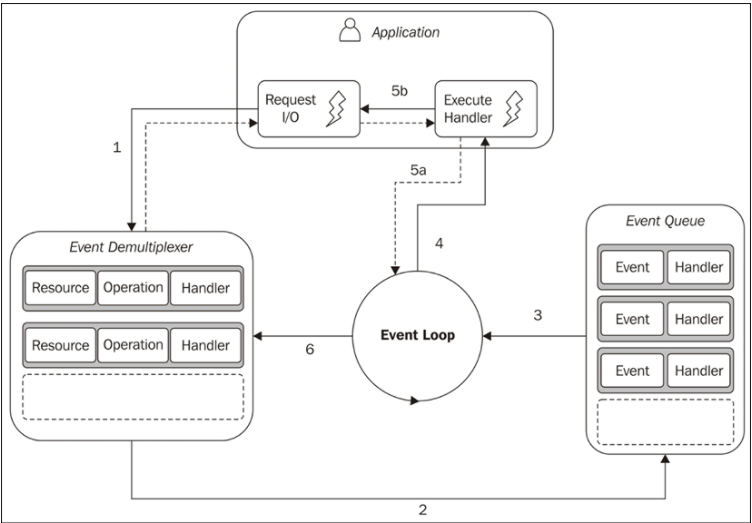
\includegraphics[width=1.0\textwidth]{reactor_pattern}
  \caption{Reactor Pattern \parencite[Abbildung 1.3]{NodeJSDesignPatterns}}
  \label{fig:reactor_pattern}
\end{figure}

Sobald die Anwendung eine I/O-Operation auf einer Ressource ausführen will, wird eine Anfrage an den
\verb|Event Demultiplexer| gestellt um diese Ressource zu beobachten.
Dabei spezifiziert die Anwendung zudem einen Handler, welcher aufgerufen wird sobald die Operation abgeschlossen wurde.
Das Verschicken einer Anfrage an den Event Demultiplexer ist ein nicht-blockierender Aufruf und gibt sofort die Kontrolle
an die Anwendung zurück.
Sobald eine I/O-Operation abgeschlossen ist und mindestens eine der beobachteten Ressourcen wieder verfügbar ist,
fügt der Event Demultiplexer die Menge an entsprechenden Events der \verb|Event Queue| hinzu.
Die \verb|Event Loop| iteriert über die Elemente der \verb|Event Queue| und ruft für jedes Event den dazugehörigen Handler auf.
Der Event-Handler, der Teil des Anwendungscodes ist, gibt die Kontrolle an die \verb|Event Loop| zurück sobald seine Ausführung
beendet ist.

Während der Event-Handler ausgeführt wird, kann dieser weitere I/O-Operationen ausführen, durch die wiederum
neue Elemente bzw. Ressourcen zum \verb|Event Demultiplexer| hinzugefügt werden.
Sobald alle Elemente in der \verb|Event Queue| verarbeitet wurden, wird die \verb|Event Loop| solange blockiert
bis der \verb|Event Queue| neue Events vom \verb|Event Demultiplexer| hinzugefügt werden (siehe Listing \ref{lst:EventLoop_Pseudocode}).
\parencite{SchmidtReactorPattern}

Das Reactor-Pattern wird unter anderem von der JavaScript-Laufzeitumgebung Node.js und vom Java-Framework \verb|Netty| implementiert.

\paragraph{Netty}

Die \verb|java.nio|-API bietet mit der Schnittstelle für \verb|Non-blocking I/O| die Grundlage für asynchrone Anwendungen.
Sie gibt aber kein Threading-Modell vor, bietet keine Unterstützung für Protokolle höherer Ebene (beispielsweise HTTP) und
kann die asynchronen I/O Events nicht verarbeiten, weswegen Entwickler in der Praxis selten direkt mit der \verb|java.nio|-API
konfrontiert sind.

Diese nicht trivialen Aufgaben werden auf der Basis von \verb|java.nio| durch das Client-Server Framework \verb|Netty| implementiert.
Dabei handelt es sich um ein asynchrones, ereignisgesteuertes Framework, welches
die Programmierung von hochperformanten Low-Level Netzwerk-Anwendungen, wie TCP- oder UDP-Socket Server vereinfacht, indem
es bereits eine breite Anzahl an Low-Level Protokollen und Transportmechanismen unterstützt (siehe Abbildung \ref{fig:netty}). \parencite{NettyUserAction}

Das Projekt verspricht dabei, gegenüber ähnlichen Frameworks, eine komfortable User Experience durch eine einheitliche API für
blockierende und nicht-blockierende I/O-Sockets. Das flexible und erweiterbare Event-Modell erlaubt zudem eine saubere Trennung der Zuständigkeiten.
Darüber hinaus beschränkt sich Netty nicht auf ein \verb|Single-thread|-Modell, sondern kann auch einen oder mehrere \verb|Thread pools| nutzen.

Gegenüber Frameworks die ähnliche Funktionalität bieten, allerdings auf \verb|Blocking I/O| basieren,
soll die Nutzung von Netty außerdem
in besserem Durchsatz, niedrigerer \Gls{latenz}(*) und geringerem Ressourcenverbrauch resultieren. \parencite{Netty}

\begin{figure}[h!]
  \centering
  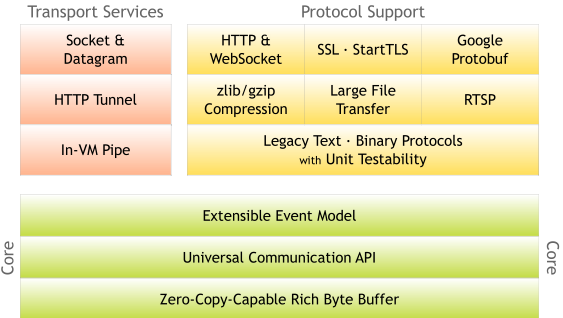
\includegraphics[width=1.0\textwidth]{netty}
  \caption{Netty Komponenten \parencite{Netty}}
  \label{fig:netty}
\end{figure}